\documentclass[fleqn,varvw,preprintnumbers,citeautoscript]{memo}

\usepackage[utf8]{inputenc}
\usepackage[T1]{fontenc}

\graphicspath{{../../fig/}}
\usepackage[caption=false]{subfig}
\usepackage{enumerate}
\usepackage{listings}


\newcommand\vlong{V_\text{long}}

\begin{document}

\title{Memo 3: schema circuitale completo}

\author{Francesco Polleri}
\email{s5025011@studenti.unige.it}
\author{Mattia Sotgia}
\email{s4942225@studenti.unige.it}

\collaboration{Gruppo A1}
\affiliation{Dipartimento di Fisica, Università degli Studi di Genova, I-16146 Genova, Italia}

\author{Lorenzo Lucentini}
\author{Michele Giorgi}
\collaboration{Gruppo C6}
\affiliation{Dipartimento di Fisica, Università degli Studi di Genova, I-16146 Genova, Italia}

\revised{\today}
\preprint{MEMO/3 (\today)}

\begin{abstract}

\end{abstract}
\maketitle

\section{I/O sistema di controllo}

\begin{enumerate}
    \item \verb-A0 (INPUT)-: lettura della tensione in uscita dall'amplificatore operazionale per strumentazione;
    \item \verb-A1 (OUTPUT)-: scrittura del valore di riferimento $V_*$ per il comparatore (deve essere compreso tra 0 V e il valore massimo assumibile (\SI{5}{\volt} (MEGA 2560) o \SI{3.3}{\volt} (DUE));
    \item \verb-D2 (GPIO/OUTPUT)-: Scrittura per avere $+$\SI{5}{\volt} (MEGA 2560) o $+$\SI{3.3}{\volt} (DUE) in uscita per alimentare il generatore di corrente.
    \item \verb-GND- collegato a terra;
    \item \verb-D14/D14_TX3 (OUTPUT/SERIAL3)-: utilizzato per la comunicazione seriale con il generatore PL303QMD-P, in ingresso al comparatore sull'input invertente. 
\end{enumerate}

\section{Logica di controllo e misura}

\begin{enumerate}
    \item chiamata a \verb-init()-;
    \item \verb-Serial.begin(9600)- e \verb-Serial3.begin(9600)-
    \item Setup \verb-I/O- pins;
    \item 
\end{enumerate}

%\begin{lstlisting}[morekeywords={init},columns=flexible]
%init();
%(Serial && Serial3).begin(9600)
%
%\end{lstlisting}


\begin{turnpage}
    \begin{figure*}[p]
        \centering
        % 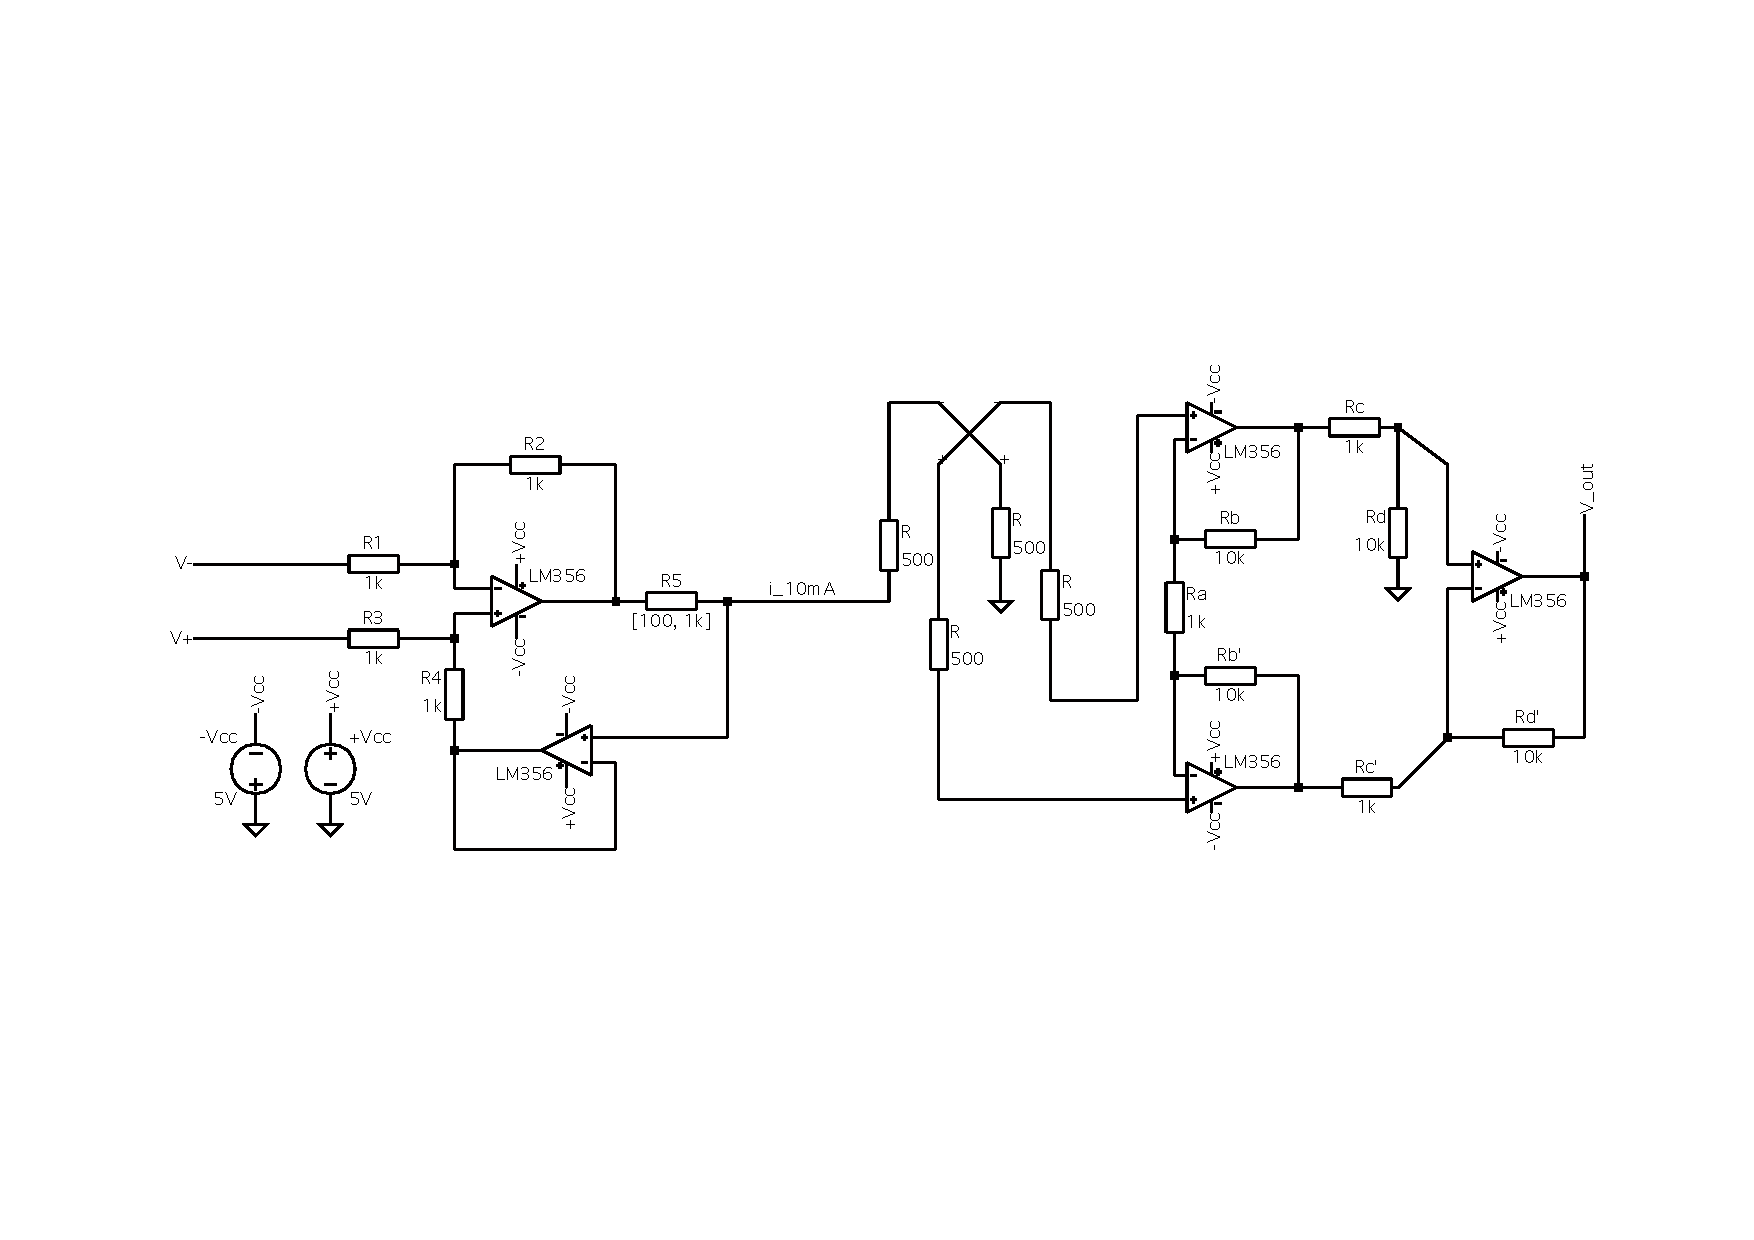
\includegraphics[width=\linewidth,trim={2cm 6.5cm 2cm 6cm},clip]{memo2_full_circuit.pdf}
        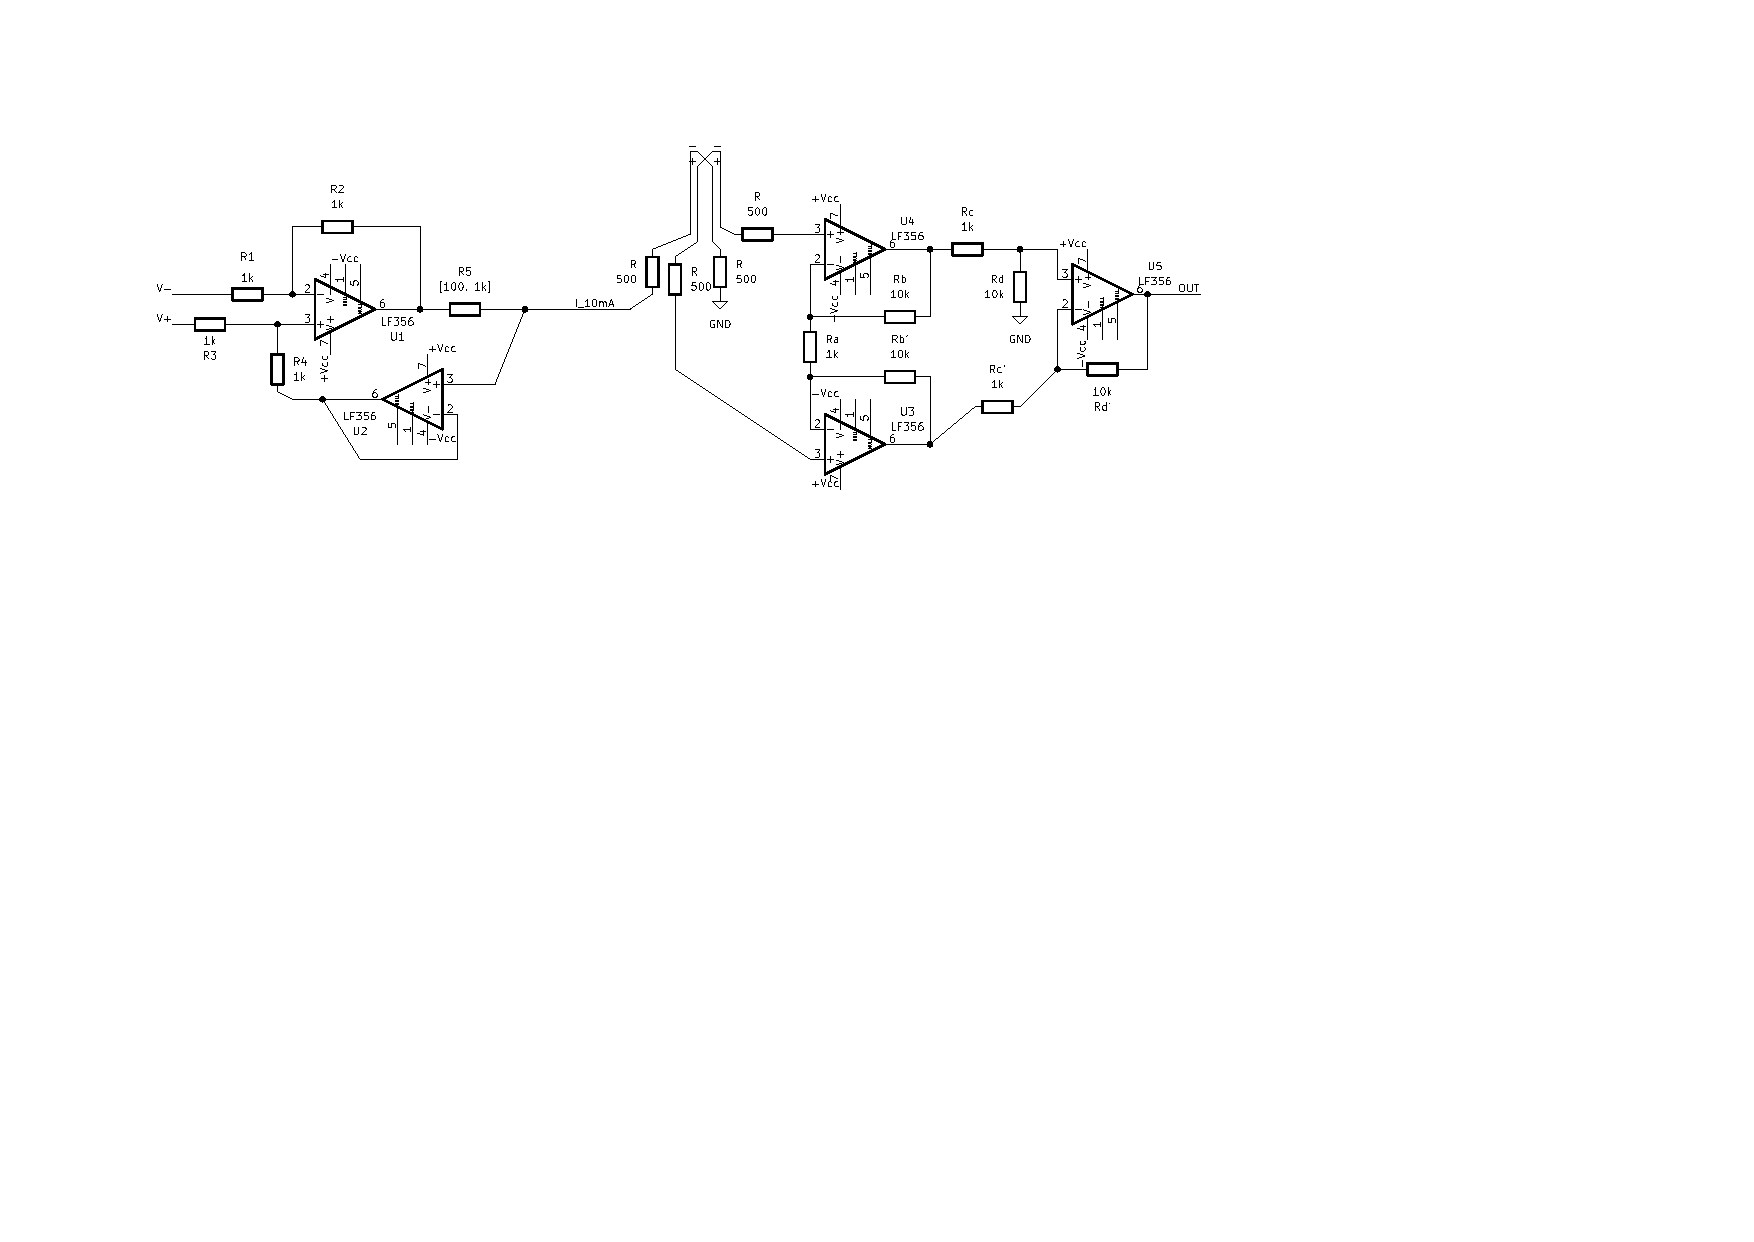
\includegraphics[width=\linewidth,trim={1.5cm 3.5cm 2cm 2cm},clip]{SCHEMA_full1.pdf}
        \caption{Circuito completo delle tre componenti principali (da sinistra a destra sono inseriti il generatore di corrente, la sonda e l'amplificatore differenziale per strumentazione). In basso a destra troviamo la scheda Arduino MEGA 2560 mappata sui pin utilizzati per il setup sperimentale. }\label{fig:circuit_memo2}
    \end{figure*}
\end{turnpage}

\end{document}